Dieses Kapitel beleuchtet dieser Arbeit zugrunde liegende Konzepte und Algorithmen. Zunächst wird das Prinzip der Epipolargeometrie beschrieben welches ein wesentlicher Bestandteil photogrammetrischer Verfahren ist. Daraufhin folgt eine Erläuterung des Terms Stereo Matching sowie eine Klassifizierung in lokale und globale Algorithmen. Im Anschluss daran wird das Prinzip des Block Matching Algorithmus grundlegend beschrieben, welcher die Grundlage für den im Rahmen dieser Arbeit verwendeten Semi Global Block Matching Algorithmus bildet. Anschließend erfolgt eine Erläuterung des verwendeten Frameworks sowie Details zur Implementierung dessen.

% ---------------------- section -----------------------
\section{Epipolargeometrie}
\label{sec:epipolargeometrie}
Bei der Verwendung der meisten photogrammetrischer Verfahren spielt die Epipolargeometrie eine entscheidende Rolle. Das mathematische Modell beschreibt die geometrische Beziehung zwischen verschiedenen Kamerabilden desselben Objektes, sowie die Abhängigkeit zwischen korrespondierenden Punkten. Generell gesehen ist die Epipolargeometrie durch das Lochkamera-Modell beschrieben. Dabei liegt jeder Punkt des aufgenommenen Objektes mit dem Projektionszentrum sowie dem Bildpunkt auf einer Geraden. Unter Zuhilfenahme der extrinsischen Orientierung sowie der intrinsischen Parameter der Kamera, ist es möglich den Schnittpunkt zweier Geraden zu berechnen um die dreidimensionalen Koordinaten des Objektpunktes zu erhalten. Dabei gilt generell, wenn ein Punkt $P$ im linken Bild gegeben ist, so wird die Suche des korrespondierenden Punktes $P’$ auf die Epipolarlinie des rechten Bildes reduziert. 

% GRAFIK: epipolargeometrie
\begin{figure}
	\begin{center}
		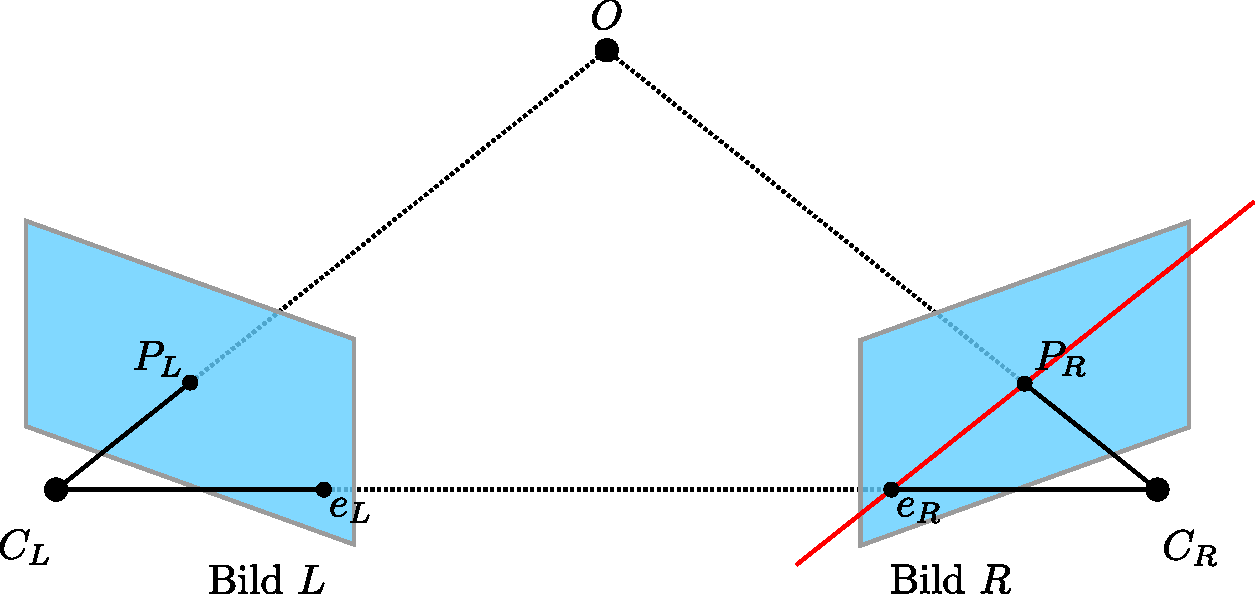
\includegraphics[width=10cm]{img/epipolar_geometry.pdf}
	\end{center}
	\caption{Darstellung der Epipolargeometrie.}
	\label{fig:epipolar_geometry}
\end{figure}

Abbildung \ref{fig:epipolar_geometry} visualisiert diesen Prozess. Gegeben sind die beiden Projektionszentren $C_L$ und $C_R$ der beiden Bildebenen sowie die Bildpunkte $P_L$ und $P_R$. Der Objektpunkt $O$ bildet im linken Kamerabild auf $P_{x_1,y_1}$ ab. Zunächst ist es nur möglich den Strahl auf welchem sich $O$ befindet zu bestimmen. Aufgrund des Wissens der extrinischen Orientierung der Kameras, können mithilfe der Basislinie zwischen den beiden Kameras die beiden Epipole in $L$ und $R$ ermittelt werden. Dabei sind diese durch den Schnittpunkt der Basislinie mit den beiden Bildebenen definiert\footnote{Im Falle eines Stereonormalfalles ist ein Schnittpunkt der Basislinie mit den Bildebenen nicht möglich, sodass die Epipole in der Unendlichkeit und parallel zur x-Achse liegen. Dies hat unter anderem den Vorteil, das die Epipolargeometrie bereits bekannt ist, und korrespondierende Bildpunkte nur noch innerhalb einer Pixelreihe gesucht werden müssen.}. Somit ist es möglich mithilfe der vorhandenen Epipole $e_L$, $e_R$ die Epipolarlinie $e_R,P_R$ zu bestimmten. Mithilfe dieser kann im Anschluss die dreidimensionale Position des Objektpunktes $O$ bestimmt werden.

% ---------------------- section -----------------------
\section{Stereo Matching}
\label{sec:stereo_matching}
Das grundlegende Konzept des Stereo Matchings beschreibt das Finden korrespondierender Punkte in zwei simultan aufgenommenen Bildern. Die Position der beiden Kameras ist dabei leicht versetzt, um einen jeweils anderen Blickwinkel auf die Szene zu erhalten. Mithilfe der verschiedenen Perspektiven können Disparitäten (Differenz der Projektion eines Objektes vom linken zum rechten Bild) zwischen korrespondierenden Pixeln berechnet werden. Die dabei erhaltenen Tiefeninformationen eines Objektes sind mit der errechneten Disparität sowie der relativen Position der Kameras, und deren intrinsischen Parametern REF, verbunden. Im Laufe dieses Prozesses kommt es zu zwei wesentlichen Problemstellungen, der Berechnung der Dispariät (Stereo Correspondence) sowie die Invertierung der Projektiven Geometrie um dreidimensionale Informationen aus der errechnetet Disparität zu erhalten. Sofern eine Lösung beider Probleme vorhanden ist können diese Informationen durch einfache Triangulierung errechnet werden.


\subsection{Klassifikation}
\label{subsec:stereo_matching_classification}
\textbf{Lokale Methoden:}\\
Zur Berechnung der Disparität in lokalen Stereo Matching Algorithen gilt grundlegendes Prinzip: “Finde Pixel $P_2$ korrespondierend zu $P_1$ im Referenzbild”. Dabei wird die Korellation von $P_1$ und $P_2$ durch deren lokale Umgebung bestimmt. Der Referenzpunkt ist dabei das Zentrum eines Bereiches in welchem das Matching ausgeführt wird. Geläufige Methoden dafür sind Sum of Absolute Differences (SAD) (Hirschmüller 2011), Zero-mean Normalized Cross-Correlation (ZNCC) (Chen \& Medioni, 1999), (Sára, 2002), Sum of Squared Differences (SSD) (Cox et al., 1996), etc.
Jedoch können aufgrund fehlender Beschränkungen verzerrte Tiefenberechnungen auftreten, da benachbarte Pixel verschiedene Disparitäten aufweisen können (beispielsweise an horizontalen Kanten wie Türrahmen etc.). Strukturell gesehen sind lokale Methoden einfacher gehalten als Globale Methoden was einen hohen Grad an Optimierung in der Implementierung zulässt.\\\\
\textbf{Globale Methoden:}\\
Bei globalen Stereo Matching Algorithmen wird ein globales Modell der zu betrachtenden Szene erstellt, sowie eine ebenfalls globale Kostenfunktion definiert, welche minimal gehalten werden soll. Dabei werden im Gegensatz zu lokalen Methoden Matches in einer Reihe und des gesamten Bildes verglichen. Zusätzlich zu den benachbarten Pixeln werden hier ebenfalls die Matches der angrenzenden Pixel betrachtet. Zur Vereinfachung dieses Vorgangs betrachten einige Algorithmen nur die Epipolargeometrie, wobei ein zweidimensionales Problem auf ein eindimensionales reduziert wird. Resultierend daraus liegt die Stärke globaler Methoden in der Bewältigung schwacher Texturen sowie auftretende Okklusionen und unterschiedlicher Lichteinfälle, was, aufgrund der höheren Komplexität in einem höheren Rechen- und Speicheraufand mündet. Weitere Verbesserungen der Ergebnisse können durch Techniken wie Dynamische Programmierung und Graph Cut erreicht werden.

\subsection{Block Matching}
\label{subsec:stereo_matching_bm}
Einen der einfachsten Ansätze zur Berechnung von Korrespondenz zwischen zwei Bildern bietet der Block Matching Algorithmus. Bei diesem lokalen Matching Algorithmus werden Blöcke bestimmter Größe mithilfe mathematischer Berechnungen (NCC, SAD, etc.)auf Korrespondenz untersucht. Dabei reduziert die Epipolargeometrie diesen Prozess auf ein eindimensionales Problem indem ein Block im linken Bild mit einem Block im rechten Bild auf der Epipolarlinie des rechten Bildes pixelweise vergleichen wird. Das eigentliche Matching erfolgt über die Berechnung eines Blockes mithilfe einer Energiefunktion. Dabei gilt es bei der Korrespondenzanalyse mit dem möglichst gleichen Wert zu erhalten. 

\begin{figure}
	\begin{center}
%		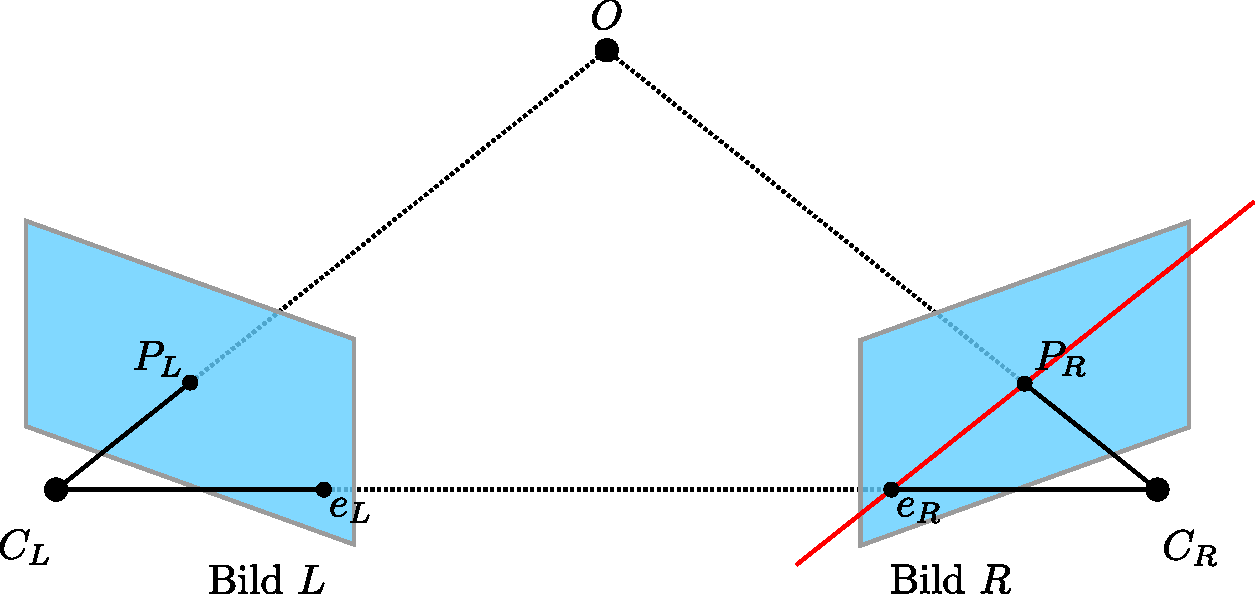
\includegraphics[width=10cm]{img/epipolar_geometry.pdf}
	\end{center}
	\caption{Visualisierung des Block Mathching Algorithmus}
	\label{fig:block_matching}
\end{figure}

\noindent
Diesen Prozess veranschaulicht Abbildung \ref{fig:block_matching}. Durch den Fokus auf einzelne Pixelreihen und deren unmittelbare Umgebung ist dieses Verfahren wesentlich schneller aber auch ungenauer als globale Matching Algorithmen. 


\subsection{Semi Global Block Matching}
\label{subsec:stereo_matching_sgbm}
Das im Rahmen dieser Arbeit verwendete Verfahren zur Berechnung von Disparity Maps ist der in der freien Computer Vision Library implementierte Semi Global Block Matching Algorithmus. Diese leicht abgewandelte Implementierung des Semi Global Matching Algorithmus von Hirschmüller et. al \cite{hirschmuller2005sgm} zeichnet sich sowohl durch seine Genauigkeit, als auch durch seine performante Berechnung aus. Unter Zuhilfenahme dieses Verfahren ist es möglich Disparity Maps in Echtzeit, mit sehr guter Framerate, zu berechnen. Im folgenden wird die grundlegende Funktionsweise des SGM erläutert. Im Anschluss daran werden die Unterschiede zum SGBM herausgearbeitet, sowie eine kurze Erklärung der Parameter dessen vorgenommen.


% ---------------------- section -----------------------
\section{mvStereoVision Framework}
\label{sec:framework}
